% compile with pdflatex -shell-escape file.tex
\documentclass[convert={density=300,outext=.png}]{standalone}
\usepackage{tikz}
\usetikzlibrary{calc,fit,positioning}
\usetikzlibrary{decorations.markings}
\usetikzlibrary{backgrounds}

% Fitting node
\makeatletter
\tikzset{
  fitting node/.style={
    inner sep=0pt,
    fill=none,
    draw=none,
    reset transform,
    fit={(\pgf@pathminx,\pgf@pathminy) (\pgf@pathmaxx,\pgf@pathmaxy)}
  },
  reset transform/.code={\pgftransformreset}
}
\makeatother

% Arrow in the middle of a path
\tikzset{->-/.style={decoration={
    markings,
    mark=at position .55 with {\arrow{>}}},postaction={decorate}}}
\tikzset{-<-/.style={decoration={
    markings,
    mark=at position .45 with {\arrow{<}}},postaction={decorate}}}


% Usage: \pipe{west coord}{east coord}{name}
\newcommand{\pipe}[3]{
    \pgfmathsetmacro{\pipeR}{0.3} % pipe radius
    \pgfmathsetmacro{\arrowSpacingCoef}{0.4} % controls the spacing of the arrows

    % Pipe drawing
    \draw
        (#1) ellipse (0.1 and \pipeR)
        ($ (#2) - (0,\pipeR) $) arc (-90:90:0.1 and \pipeR)
        ($ (#1) + (0,\pipeR) $) -- ($ (#2) + (0,\pipeR) $)
        ($ (#1) - (0,\pipeR) $) -- ($ (#2) - (0,\pipeR) $)
        node[fitting node] (#3) {};

    % Arrows inside pipe
    \draw[->-,dashed,color=gray]
        ($ (#1) + (0.1,\pipeR*\arrowSpacingCoef) $) -- ($ (#2) + (0.1,\pipeR*\arrowSpacingCoef) $)
        coordinate[pos=0] (#3 west in) coordinate[pos=1] (#3 east out);
    \draw[-<-,dashed,color=gray]
        ($ (#1) + (0.1,-\pipeR*\arrowSpacingCoef) $) -- ($ (#2) + (0.1,-\pipeR*\arrowSpacingCoef) $)
        coordinate[pos=0] (#3 west out) coordinate[pos=1] (#3 east in);
}

% Usage: \iobox{pos}{width}{height}{n_west}{n_east}{name}{label}
\newcommand{\iobox}[7]{
    \draw (#1) node[rectangle, draw, minimum width=#2, minimum height=#3] (#6) {#7};

    % West anchors
    \pgfmathsetmacro{\n}{#4-1}
    \foreach \ii in{0,1,...,\n}{
        \pgfmathsetmacro{\pos}{(\ii+1)/(#4+1)}
        \path (#6.north west)--(#6.south west) coordinate[pos=\pos] (#6 west\ii);
    }

    % East anchors
    \pgfmathsetmacro{\n}{#5-1}
    \foreach \ii in{0,1,...,\n}{
        \pgfmathsetmacro{\pos}{(\ii+1)/(#5+1)}
        \path (#6.north east)--(#6.south east) coordinate[pos=\pos] (#6 east\ii);
    }
}

\begin{document}
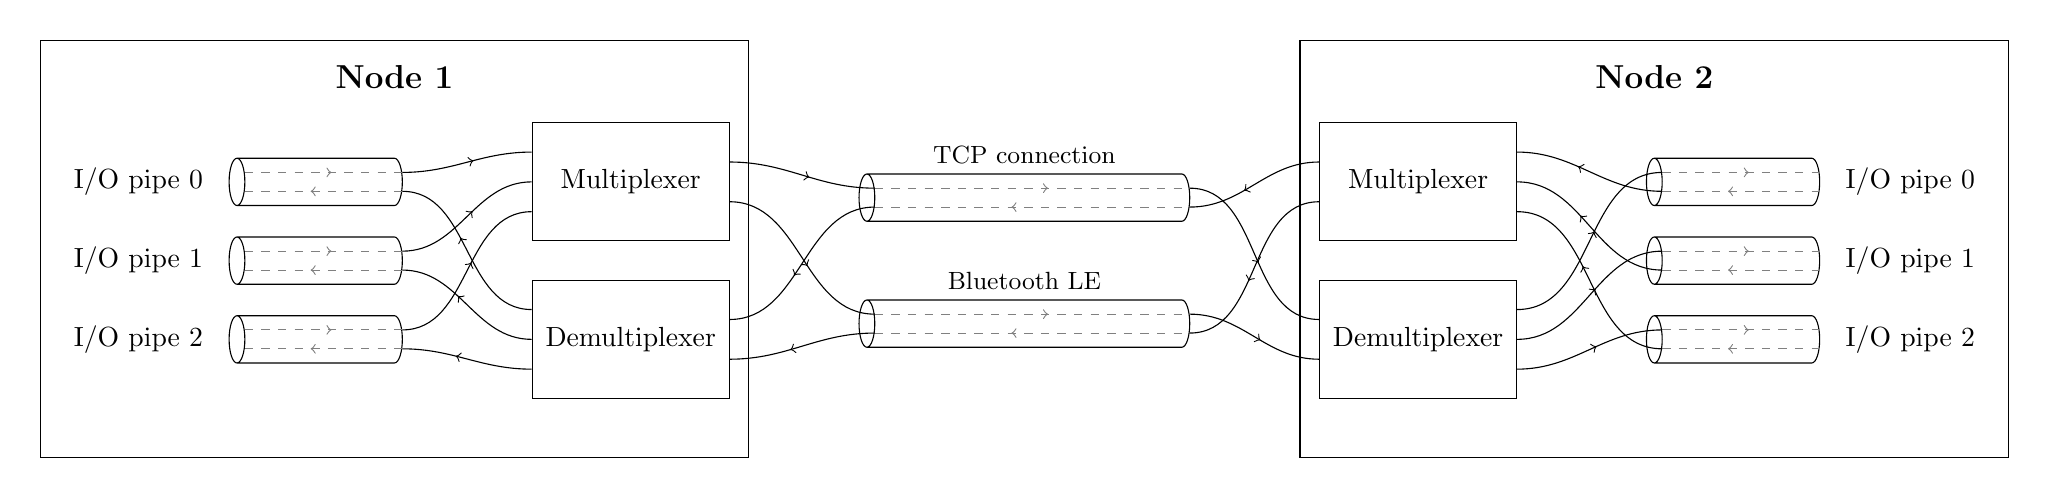
\begin{tikzpicture}[background rectangle/.style={fill=white!45}, show background rectangle]
    \pgfmathsetmacro{\nodedist}{5}
    \pgfmathsetmacro{\channelL}{0.3}

    \pgfmathsetmacro{\pipeS}{8}
    \pgfmathsetmacro{\pipeE}{10}

    \pgfmathsetmacro{\channelAH}{0.8}
    \pgfmathsetmacro{\channelBH}{-0.8}

    % Mux/demux left
    \iobox{-\nodedist,1}{2.5cm}{1.5cm}{3}{2}{mux1}{Multiplexer}
    \iobox{-\nodedist,-1}{2.5cm}{1.5cm}{3}{2}{demux1}{Demultiplexer}

    % Mux/demux right
    \iobox{\nodedist,1}{2.5cm}{1.5cm}{2}{3}{mux2}{Multiplexer}
    \iobox{\nodedist,-1}{2.5cm}{1.5cm}{2}{3}{demux2}{Demultiplexer}

    % Channel 0
    \pipe{-\nodedist+3,\channelAH}{\nodedist-3,\channelAH}{channel0}
    \draw node[above=0 of channel0] {\small TCP connection};
    \draw (mux1 east0) edge[->-,out=0,in=180] (channel0 west in);
    \draw (demux1 east0) edge[-<-,out=0,in=180] (channel0 west out);
    \draw (channel0 east in) edge[-<-,out=0,in=180] (mux2 west0);
    \draw (channel0 east out) edge[->-,out=0,in=180] (demux2 west0);

    % Channel 1
    \pipe{-\nodedist+3,\channelBH}{\nodedist-3,\channelBH}{channel1}
    \draw node[above=0 of channel1] {\small Bluetooth LE};
    \draw (mux1 east1) edge[->-,out=0,in=180] (channel1 west in);
    \draw (demux1 east1) edge[-<-,out=0,in=180] (channel1 west out);
    \draw (channel1 east in) edge[-<-,out=0,in=180] (mux2 west1);
    \draw (channel1 east out) edge[->-,out=0,in=180] (demux2 west1);

    % I/O Pipes left
    \pgfmathsetmacro{\pipeAH}{1}
    \pgfmathsetmacro{\pipeBH}{0}
    \pgfmathsetmacro{\pipeCH}{-1}
    \pipe{-\pipeE,\pipeAH}{-\pipeS,\pipeAH}{iopipe10}
    \draw node[left=0.2 of iopipe10] {I/O pipe 0};
    \draw (iopipe10 east out) edge[->-,out=0,in=180] (mux1 west0);
    \draw (iopipe10 east in) edge[-<-,out=0,in=180] (demux1 west0);
    \pipe{-\pipeE,\pipeBH}{-\pipeS,\pipeBH}{iopipe11}
    \draw node[left=0.2 of iopipe11] {I/O pipe 1};
    \draw (iopipe11 east out) edge[->-,out=0,in=180] (mux1 west1);
    \draw (iopipe11 east in) edge[-<-,out=0,in=180] (demux1 west1);
    \pipe{-\pipeE,\pipeCH}{-\pipeS,\pipeCH}{iopipe12}
    \draw node[left=0.2 of iopipe12] {I/O pipe 2};
    \draw (iopipe12 east out) edge[->-,out=0,in=180] (mux1 west2);
    \draw (iopipe12 east in) edge[-<-,out=0,in=180] (demux1 west2);

    % I/O Pipes right
    \pipe{\pipeS,\pipeAH}{\pipeE,\pipeAH}{iopipe20}
    \draw node[right=0.2 of iopipe20] {I/O pipe 0};
    \draw (mux2 east0) edge[-<-,out=0,in=180] (iopipe20 west out);
    \draw (demux2 east0) edge[->-,out=0,in=180] (iopipe20 west in);
    \pipe{\pipeS,\pipeBH}{\pipeE,\pipeBH}{iopipe21}
    \draw node[right=0.2 of iopipe21] {I/O pipe 1};
    \draw (mux2 east1) edge[-<-,out=0,in=180] (iopipe21 west out);
    \draw (demux2 east1) edge[->-,out=0,in=180] (iopipe21 west in);
    \pipe{\pipeS,\pipeCH}{\pipeE,\pipeCH}{iopipe22}
    \draw node[right=0.2 of iopipe22] {I/O pipe 2};
    \draw (mux2 east2) edge[-<-,out=0,in=180] (iopipe22 west out);
    \draw (demux2 east2) edge[->-,out=0,in=180] (iopipe22 west in);

    
    \pgfmathsetmacro{\nodeNorth}{2.8}
    \pgfmathsetmacro{\nodeSouth}{-2.5}
    \pgfmathsetmacro{\nodeS}{\nodedist-1.5}
    \pgfmathsetmacro{\nodeE}{\pipeE+2.5}
    \draw (-\nodeE,\nodeNorth) rectangle (-\nodeS,\nodeSouth) node[fitting node] (node1) {};
    \draw node[below=0.2 of node1.north] {\large\bf Node 1};
    \draw (\nodeS,\nodeNorth) rectangle (\nodeE,\nodeSouth) node[fitting node] (node2) {};
    \draw node[below=0.2 of node2.north] {\large\bf Node 2};
\end{tikzpicture}
\end{document}